\documentclass[11pt]{article}
\usepackage[margin=1in]{geometry}
\usepackage{amsmath,amssymb,graphicx,booktabs,hyperref,xcolor,enumitem,listings}
\hypersetup{colorlinks=true,linkcolor=blue!50!black,urlcolor=blue!50!black,citecolor=blue!50!black}
\lstset{basicstyle=\ttfamily\small,breaklines=true,frame=single,columns=fullflexible}
\newcommand{\todo}[1]{\textcolor{red}{[TODO: #1]}}
\newcommand{\tbd}{\textcolor{red}{\textbf{TBD}}}

\title{Single-Image Refocusing with a Fine-Tuned Video Diffusion Model:\\
Reproduction and a Controlled Conditioning Ablation}
\author{Bhavya \\ \textit{Final project, course name \todo{fill in}}}
\date{\today}

\begin{document}
\maketitle

\begin{abstract}
Given one photograph with an arbitrary focus setting, we want to produce a \emph{focal stack}---the same scene
at several focus distances---so that a user can click any pixel and bring it into focus.
We follow Tedla et al.~\cite{tedla2025refocus}, who treat a focal stack as a video and fine-tune
Stable Video Diffusion~\cite{blattmann2023svd} on a smartphone focal-stack dataset.
We (i) reproduce their pipeline and evaluate their released checkpoint, (ii) fine-tune the same
model ourselves under a small compute budget, and (iii) run a controlled ablation on how the input image and its focus position are presented to the network.
\tbd{one-sentence headline result}.
\end{abstract}

\section{Problem statement}
A thin-lens camera focused at distance $d_f$ renders a point at depth $z$ with a blur circle whose diameter grows with $|1/z - 1/d_f|$.
Blur destroys information, so recovering a sharp image, or an image focused elsewhere, from a single photo is ill-posed:
many sharp scenes are consistent with the same blurry observation.
This favours a \emph{generative} model that samples plausible detail over a regression model that averages it away.

\textbf{Task.} Input: one RGB image $I_k$ captured at (known) focal position $k\in\{0,\dots,8\}$.
Output: a stack $\{\hat I_0,\dots,\hat I_8\}$ of nine images of the same scene, one per focal position.
\textbf{Interface.} The user clicks pixel $p$; we return the frame $\hat I_{j^\star}$ that is sharpest in a window around $p$ (Section~\ref{sec:ui}).

\section{Background and model choices}
\subsection{Why a video model?}
Moving the focal plane changes the image smoothly and consistently: geometry and colour stay fixed while blur varies.
That is the same structure as a video, where content persists across frames while some factor changes.
A pretrained video diffusion model already encodes strong priors for (a) realistic image appearance and (b) temporal consistency, so
we only need to teach it that ``time'' now means ``focus distance''.
This is far cheaper than training an image-to-stack network from scratch, which would need orders of magnitude more data and compute than our budget (\$100) allows.

\subsection{Stable Video Diffusion (SVD)}
We start from \texttt{stabilityai/stable-video-diffusion-img2vid} (the weights downloaded by the authors' \texttt{setup/download\_svd\_weights.py}).
It is a \emph{latent} diffusion model with three parts, each of which appears in the training code (\texttt{training/svd\_runner.py}):
\begin{itemize}[noitemsep]
  \item \textbf{VAE} (\texttt{AutoencoderKLTemporalDecoder}): maps each frame to a $4$-channel latent at $1/8$ spatial resolution. \emph{Frozen.}
  \item \textbf{CLIP image encoder} (\texttt{CLIPVisionModelWithProjection}): embeds the conditioning image into a vector used through cross-attention. \emph{Frozen.}
  \item \textbf{Denoising U-Net} (\texttt{UNetSpatioTemporalConditionModel}): residual convolution blocks and transformer blocks that operate per frame
        (``spatial'' layers) and across frames (``temporal'' layers). \emph{Partly trained} (below).
\end{itemize}
\todo{add architecture figure (TikZ) showing VAE / CLIP / U-Net and where the conditioning enters}

\subsection{Diffusion objective (EDM parameterisation)}
SVD uses the EDM framework of Karras et al.~\cite{karras2022edm}. Given clean latents $x_0$ and noise level $\sigma$, the network sees $x_\sigma = x_0 + \sigma\epsilon$.
The training code implements:
\begin{align}
  \sigma &\sim \text{LogNormal}(P_{\text{mean}}{=}0.7,\ P_{\text{std}}{=}1.6),\\
  \text{net input} &= x_\sigma / \sqrt{\sigma^2+1}, \qquad t = \tfrac14 \log\sigma,\\
  D_\theta(x_\sigma) &= c_{\text{skip}}\,x_\sigma + c_{\text{out}}\,F_\theta, \quad
     c_{\text{skip}}=\tfrac{1}{\sigma^2+1},\ c_{\text{out}}=\tfrac{-\sigma}{\sqrt{\sigma^2+1}},\\
  \mathcal{L} &= \mathbb{E}\Big[\, \tfrac{1+\sigma^2}{\sigma^2}\ \lVert D_\theta(x_\sigma) - x_0 \rVert_2^2 \Big].
\end{align}
The loss is a mean squared error in \emph{latent} space, weighted so that all noise levels contribute comparably.

\section{Our model: what is fine-tuned and how}
\subsection{Representing a focal stack as a 9-frame video}
Frame $j$ of the ``video'' is the photo focused at position $j$ (position $0$ is nearest, about 5\,cm; position $8$ is infinity, following the repository README).
We set \texttt{num\_frames}\,=\,9.

\subsection{Conditioning on the input photo}
At each training step one frame index $k$ is drawn uniformly from $\{0,\dots,8\}$ and treated as the observed input (conditioning mode \texttt{random}).
Two signals tell the network about it:
\begin{enumerate}[noitemsep]
  \item \textbf{Channel concatenation.} The VAE latent of frame $k$ is placed at temporal slot $k$; all other slots are set to zero (a binary mask over frames).
        This $4$-channel tensor is concatenated with the $4$-channel noisy latent, so the U-Net input has $8$ channels. \emph{The position of the non-zero slot encodes which focus position the input has.}
  \item \textbf{Cross-attention.} The CLIP embedding of frame $k$ is supplied as the (single-token) context.
\end{enumerate}
Following SVD we also add small Gaussian noise to the conditioning image (noise-augmentation level drawn from LogNormal$(-3.0,0.5)$) and, with probability $0.1$ each,
drop the image latent or the CLIP embedding to enable classifier-free guidance at inference.

\subsection{What is trained}
Only the parameters whose names contain \texttt{temporal\_transformer\_block} are updated; everything else (VAE, CLIP, spatial convolutions, spatial attention) is frozen.
Rationale: the \emph{spatial} layers already model how a single image looks. What must change is how frames relate to each other, which is exactly the job of the temporal layers.
This keeps the optimiser state small and limits overfitting on a modest dataset.
\todo{report exact trainable parameter count / percentage once measured on the GPU}

\begin{table}[h]\centering
\caption{Training hyperparameters taken from \texttt{configs/focal\_stacks\_train.yaml} (authors' defaults).}
\begin{tabular}{ll}\toprule
Optimiser & AdamW, $\beta=(0.9,0.999)$, weight decay 0.01\\
Learning rate & $10^{-5}$ constant (\texttt{scale\_lr: true}), no warm-up\\
Batch size & 1 per GPU\\
Precision & fp32 weights (\texttt{mixed\_precision: null}), TF32 off\\
Frames / resolution & 9 frames, $640\times896$ px ($80\times112$ latent)\\
Conditioning dropout & 0.1\\
EMA & off\\
Checkpoint released by authors & 200{,}000 steps\\
\bottomrule\end{tabular}
\end{table}

\section{Data and preprocessing}
\textbf{Dataset.} Tedla et al.\ release smartphone focal stacks with $9$ focal positions per scene, in three variants: raw DNG, full-resolution undistorted, and
\emph{midsize undistorted} ($896\times640$, centre camera only). Training and testing in the code use the midsize variant.
We use only this variant: it is the smallest, and it is the one the released code expects (\texttt{RigCenter*} folders with exactly nine \texttt{.jpg} files).
Train/test scene lists are in \texttt{splits/*.pkl}; the test split has 164 scenes (from the metric script).
\textbf{What we downloaded and verified.} The file \texttt{scenes\_merged\_midsize\_undistorted\_RigCenter.zip} (943.8\,MB on the share, 7.3\,GB extracted)
contains 1{,}643 scene folders and 14{,}764 JPEGs, each $640\times896$ (width $\times$ height).
Of these, 1{,}638 scenes have all nine focal positions; five folders are incomplete (1, 2, 4, 7 and 8 frames) and belong to no split, so they are never used.
The split files (\texttt{train\_scenes.pkl}, \texttt{test\_scenes.pkl}) are byte-identical between the repository and the \texttt{splits.zip} on the share:
\textbf{1{,}474 training scenes and 164 test scenes, with no overlap}, all complete. Scenes are dated across 17 capture days between August and December 2024.
\todo{capture device, licence of the dataset}

\textbf{Preprocessing log (everything we did to the data).}
\begin{enumerate}[noitemsep]
  \item Downloaded the single \texttt{midsize\_undistorted\_RigCenter} archive and \texttt{splits.zip} (the full-size and DNG archives are 17--51\,GB each and are not used).
  \item Verified frame counts and split membership per scene (script \texttt{scripts/dataset\_stats.py}).
  \item \textbf{Windows file-name issue:} scene names contain a colon (\texttt{GMT-05:00}), which Windows replaces with an underscore on extraction, so split lists no longer match folder names on a Windows machine. We therefore extract on the Linux training machine, where the names are preserved.
  \item No other modification: no cropping, no colour change, no augmentation beyond what the training code does (resize to $640\times896$, which is a no-op here, and scaling to $[-1,1]$).
\end{enumerate}

\textbf{Preprocessing (from \texttt{FocalStackDataset}).}
\begin{enumerate}[noitemsep]
  \item Keep only folders containing exactly 9 frames.
  \item Sort the frames by file name to obtain focal order $0,\dots,8$.
  \item Resize to $640\times896$ (width\,$\times$\,height), convert to float, and rescale pixel values from $[0,255]$ to $[-1,1]$ (the VAE's input range).
  \item Encode every frame with the frozen VAE and multiply by the VAE scaling factor to get latents $x_0\in\mathbb{R}^{9\times4\times112\times80}$.
\end{enumerate}
Note that the dataset class resizes with plain \texttt{PIL.resize}; the images are already midsize so this is nearly a no-op.
\todo{augmentation: none observed in code; confirm}

\section{Experiments}
\subsection{Baseline: authors' released checkpoint}
We run the 200k-step checkpoint (\texttt{tedlasai/learn2refocus} on Hugging Face, 15.4\,GB) on the test split. \tbd

\subsection{Our fine-tune and the ablation}
The training script already supports several conditioning modes (\texttt{conditioning:} in the YAML):
\texttt{random}, \texttt{zero}, \texttt{ablate\_position}, \texttt{ablate\_time}, \texttt{ablate\_single\_frame}, \texttt{random\_single\_double\_triple}.
An \emph{ablation} changes exactly one factor while keeping data, steps, seed and hyperparameters identical, so any difference in quality is attributable to that factor.
\todo{choose the compared modes, e.g.\ \texttt{random} vs.\ \texttt{ablate\_position}; document what each does after reading the code in detail}

\begin{table}[h]\centering
\caption{Test-set metrics (mean over 164 scenes). \tbd}
\begin{tabular}{lccccc}\toprule
Model & PSNR$\uparrow$ & SSIM$\uparrow$ & LPIPS$\downarrow$ & FID$\downarrow$ & VIF$\uparrow$\\\midrule
Authors' 200k ckpt & \tbd & \tbd & \tbd & \tbd & \tbd\\
Ours, mode A & \tbd & \tbd & \tbd & \tbd & \tbd\\
Ours, mode B & \tbd & \tbd & \tbd & \tbd & \tbd\\
\bottomrule\end{tabular}
\end{table}
Metrics follow the authors' \texttt{extra/compute\_metrics.py}: PSNR, SSIM, LPIPS (VGG), FID and VIF, computed for every (input position, output position) pair.

\subsection{Compute budget}
\tbd{GPU type, hours, cost per run, total spent versus the \$100 cap}

\section{Click-to-refocus interface}\label{sec:ui}
Given the generated stack, define a local sharpness for frame $j$ at pixel $p$, e.g.\ the variance of the Laplacian in a window $W_p$:
$s_j(p)=\mathrm{Var}_{q\in W_p}[\nabla^2 \hat I_j(q)]$. Clicking $p$ displays $\hat I_{j^\star}$ with $j^\star=\arg\max_j s_j(p)$.
\todo{implement, show screenshots, discuss failure on textureless regions}


\section{Extra credit: depth and focus (exploration)}\label{sec:depth}
\textbf{Idea.} In a focal stack, the frame that is sharpest at a pixel is a proxy for that pixel's depth (depth from focus). If so, a monocular depth estimator should \emph{agree} with the focal stack, and depth could be used to evaluate, calibrate, or condition a refocusing model.

\textbf{Experiment (real data, no training).} For 16 test scenes (every $\sim$10th scene in \texttt{test\_scenes.pkl}) we computed (i) the per-pixel index of the sharpest frame (absolute Laplacian, $21\times21$ box filter) and (ii) relative disparity from Depth Anything V2 Small~\cite{yang2024depthanythingv2} on the middle frame (position 4). Using the 40\% most textured pixels with a clear sharpness peak, we measured the Spearman rank correlation between the two.
\begin{figure}[h]\centering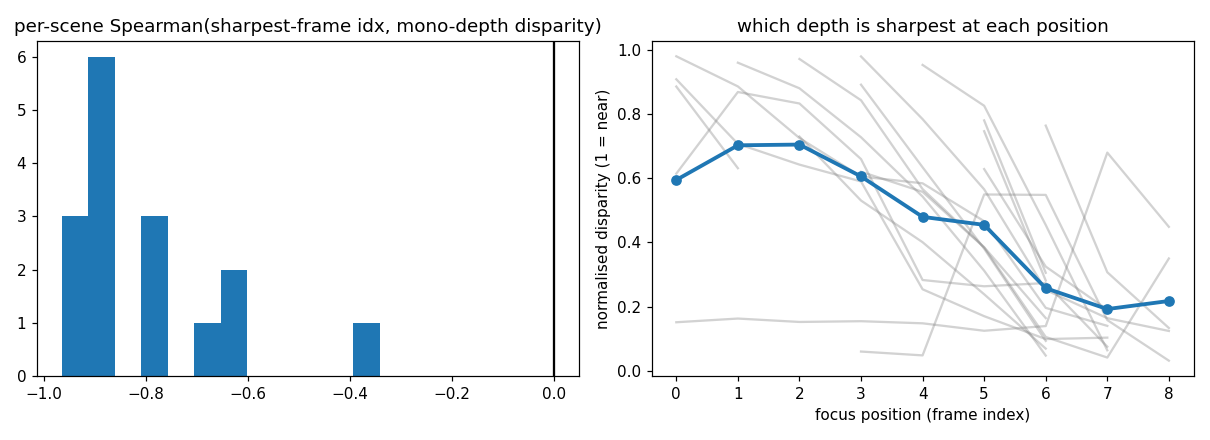
\includegraphics[width=\linewidth]{depth_vs_focus.png}
\caption{Left: per-scene Spearman correlation between the sharpest-frame index and monocular disparity (mean $-0.80$; all 16 scenes negative, range $-0.97$ to $-0.35$). Right: median normalised disparity (1 = near) of pixels that are sharpest at each focus position; light lines are single scenes.}\end{figure}
\textbf{Result.} Near pixels are sharpest at low positions and far pixels at high positions, as expected (mean $\rho=-0.80$). The mean curve is roughly flat over positions 0--2 and then falls steadily to position 8.
\textbf{Caveats.} One depth model, 16 scenes, a hand-chosen texture mask, relative (not metric) depth, and only ``which depth is sharp'' not absolute distance. It is an exploration, not a benchmark.

\textbf{Opportunities we considered} (ordered by effort/benefit): (A) a label-free \emph{depth-consistency score} for generated stacks, i.e.\ the same correlation computed on the model's output; (B) a classical baseline (monocular depth + synthetic lens blur) to show what a generative model adds, namely sharpening and not only blurring; (C) depth as an extra conditioning input or an auxiliary loss, which is the riskiest because it changes the network input; (D) NYU Depth V2~\cite{silberman2012nyu} (1{,}449 labelled RGB-D pairs, 2.8\,GB) to validate the depth estimator or to simulate focal stacks, with the caveats of Kinect depth holes, low resolution and no stated licence; (E) using the measured position--depth relationship to place objects in the Blender demo so it matches the phone's scale.

\section{Limitations and discussion}
\tbd

\section{Conclusion}
\tbd

\begin{thebibliography}{9}
\bibitem{tedla2025refocus} S.~Tedla, Z.~Zhang, X.~Zhang, S.~Xin. \emph{Learning to Refocus with Video Diffusion Models}. ACM SIGGRAPH Asia, 2025.
  \url{https://learn2refocus.github.io/}; code: \url{https://github.com/tedlasai/learn2refocus}.
\bibitem{blattmann2023svd} A.~Blattmann et al. \emph{Stable Video Diffusion: Scaling Latent Video Diffusion Models to Large Datasets}. arXiv:2311.15127, 2023.
\bibitem{karras2022edm} T.~Karras, M.~Aittala, T.~Aila, S.~Laine. \emph{Elucidating the Design Space of Diffusion-Based Generative Models}. NeurIPS, 2022.
\bibitem{yang2024depthanythingv2} L.~Yang et al. \emph{Depth Anything V2}. NeurIPS, 2024. arXiv:2406.09414.
\bibitem{silberman2012nyu} N.~Silberman, D.~Hoiem, P.~Kohli, R.~Fergus. \emph{Indoor Segmentation and Support Inference from RGBD Images}. ECCV, 2012. \url{https://cs.nyu.edu/~fergus/datasets/nyu_depth_v2.html}.
\end{thebibliography}
\end{document}
